%@TheDoctorRAB
%standard white paper/preproposal format
%
%%%%%
%
%REFERENCES
%
%neup.bst - numbered citations in order of appearance, short author list with et al in reference section
%nsf.bst - numbered citations in order of appearance, full author list in references section
%standard.bst - citations with author last name with et al for more than 2 authors; full author list in references section
%ans.bst is for ANS only. 
%
%author = {Lastname, Firstname and Lastname, Firstname and Lastname, Firstname} for all bst formats
%bst renders the author list itself
%
%author = {{Nuclear Regulatory Commission}} if the author is an organization, institution, etc., and not people
%
%title = {{}} for all
%
%for all - use \citep{-} - [1] or (Borrelli, 2021) in the text
%standard.bst \cite{-} - Borrelli (2021) in the text
%standard.bst lists references alphabetically
%the rest list numerically
%
%
%%% slides 
%
%\citep{xxxnna} where the citation should go
%\blfootnote{\fontsize\cite{xxxnna}\fontsize\bibentry{xxxnna}} before \end{frame}
%
%
%%%%%

%%%%% presentation settings
\documentclass[aspectratio=1610,pdftex,dvipsnames,compress,xcolor={dvipsnames}]{beamer}
\usetheme{Boadilla}
\usecolortheme{seahorse}
\beamertemplatenavigationsymbolsempty
\addtobeamertemplate{footnote}{\hskip -2em}{} %pushes footnote to margin
\setbeamerfont{title}{series=\bfseries}
\setbeamertemplate{page number in head/foot}[framenumber] %just gives slide number; comment out for 1/7, 2/7...
\definecolor{BackGround}{RGB}{255,250,240}
\setbeamercolor{background canvas}{bg=BackGround}
%%%%%


%%%%% general 
%\documentclass[11pt,a4paper]{article}
%\usepackage[lmargin=1in,rmargin=1in,tmargin=1in,bmargin=1in]{geometry}
\usepackage[pagewise]{lineno} %line numbering
\usepackage{setspace}
\usepackage{ulem} %strikethrough - do not \sout{\cite{}}
\usepackage{graphicx}
\usepackage{mypythonhighlight,verbatim}
\usepackage{filecontents}
\usepackage{tablefootnote}
\usepackage{footnotehyper}
\usepackage{float}
%\usepackage{subfig}
\usepackage[yyyymmdd]{datetime} %date format
\renewcommand{\dateseparator}{.}
\graphicspath{{img/}} %path to graphics
\setcounter{secnumdepth}{5} %set subsection to nth level
\usepackage{needspace}
\usepackage[stable,hang,flushmargin]{footmisc} %footnotes in section titles and no indent; standard.bst
\usepackage[inline]{enumitem}
\setlist[itemize]{label=\textbullet}
\usepackage{boldline}
\usepackage{makecell}
\usepackage{booktabs}
\usepackage{amssymb}
\usepackage{gensymb}
\usepackage{amsmath,nicefrac}
\usepackage{physics}
\usepackage{lscape}
\usepackage{array}
\usepackage{chngcntr}
\usepackage{hyperref}
\hypersetup{colorlinks,linkcolor=black,citecolor=black,urlcolor=blue} 
%\usepackage{sectsty}
\usepackage{textcomp}
\usepackage{lastpage}
\usepackage{xargs} %for \newcommandx
\usepackage[colorinlistoftodos,prependcaption,textsize=tiny]{todonotes} %makes colored boxes for commenting
\usepackage{soul}
\usepackage{color}
\usepackage{marginnote}
\usepackage[figure,table]{totalcount}
\usepackage[capitalise]{cleveref}
\usepackage{microtype} %improves typography for pdf
\usepackage[pdftex,dvipsnames]{colortbl} %change font color
%%%%%


%%%%% tikz
\usepackage{pgf}
\usepackage{tikz} % required for drawing custom shapes
\usetikzlibrary{shapes,arrows,automata,trees}
%%%%%


%%%%% fonts
\usepackage{times}
%\renewcommand{\sfdefault}{ubuntu}
%arial - uncomment next two lines
%\usepackage{helvet}
%\renewcommand{\familydefault}{\sfdefault}
%%%%%


%%%%% references
%\usepackage[round,semicolon]{natbib} %for (Borrelli 2021; Clooney 2019) - standard.bst 
\usepackage[numbers,sort&compress]{natbib} %for [1-3] - nsf.bst, neup.bst
\setlength{\bibsep}{7pt} %sets space between references
%\renewcommand{\bibsection}{} %suppresses large 'references' heading
%\renewcommand\bibpreamble{\vspace{\baselineskip}} %sets spacing after heading if not using default references heading
%%%%%


%%%%% tables and figures
\usepackage{longtable} %need to put label at top under caption then \\ - use spacing
\usepackage{tablefootnote}
\usepackage{tabularx}
\usepackage{multirow}
\usepackage{tabto} %general tabbed spacing
\usepackage{pdfpages}
\usepackage{wrapfig} %wraps figures around text
\setlength{\intextsep}{0.00mm}
\setlength{\columnsep}{1.00mm}
\usepackage[singlelinecheck=false,labelfont=bf]{caption}
\usepackage{subcaption}
\captionsetup[table]{justification=justified,skip=5pt,labelformat={default},labelsep=period,name={Table}} %sets a space after table caption
\captionsetup[figure]{justification=justified,skip=5pt,labelformat={default},labelsep=period,name={Figure}} %sets space above caption, 'figure' format
\captionsetup[wrapfigure]{justification=centering,aboveskip=0pt,belowskip=0pt,labelformat={default},labelsep=period,name={Fig.}} %sets space above caption, 'figure' format
\captionsetup[wraptable]{justification=centering,aboveskip=0pt,belowskip=0pt,labelformat={default},labelsep=period,name={Table}} %sets space above caption, 'figure' format
%%%%%


%%%%% watermark
%\usepackage[firstpage,vpos=0.63\paperheight]{draftwatermark}
%\SetWatermarkText{\shortstack{DRAFT\\do not distribute}}
%\SetWatermarkScale{0.20}
%%%%%


%%%%% cross referencing files
%\usepackage{xr} %for revisions - will cross reference from one file to here
%\externaldocument{/path/to/auxfilename} %aux file needed
%%%%%


%%%%% toc and glossaries
\usepackage[toc,title]{appendix}
\usepackage[acronym,nomain,nonumberlist]{glossaries}
\makenoidxglossaries
%\usepackage{titlesec,titletoc}
%\renewcommand{\thepart}{ARTICLE \Roman{part}} %puts the label into the command so \thelabel will carry through
%\renewcommand{\thesection}{\arabic{section}} %puts the label into the command so \thelabel will carry through
%\titleformat{\part}{\normalfont\large\bfseries}{\thepart}{}{}[]
%\titlespacing*\part{0pt}{0.95\baselineskip}{0.75\baselineskip}
%\titleformat{\section}[runin]{\normalfont\large\bfseries}{\thesection}{-1em}{}[.]
%\titlespacing*\section{0pt}{0.65\baselineskip}{0.55\baselineskip}
%\titleformat{\subsection}[runin]{\normalfont\normalsize\bfseries}{\thesubsection}{-1em}{}[.]
%\titlespacing*\subsection{0pt}{0.50\baselineskip}{0.35\baselineskip}
%\titleformat{\paragraph}[runin]{\normalfont\normalsize\bfseries\itshape}{\theparagraph}{-1em}{}[.]
%\titlespacing*\paragraph{0pt}{0.45\baselineskip}{0.25\baselineskip}
%\titleformat{\subparagraph}[runin]{\normalfont\normalsize\itshape}{\thesubparagraph}{-1em}{}[.]
%\titlespacing*\subparagraph{0pt}{0.40\baselineskip}{0.25\baselineskip}
%\titleformat{\paragraph}[hang]{\normalfont\normalsize\bfseries}{\theparagraph}{5pt}{}[]
%\titlespacing*\paragraph{0pt}{0.50\baselineskip}{0.25\baselineskip}
%\titleformat{\subparagraph}[runin]{\normalfont\normalsize\itshape}{\thesubparagraph}{-1em}{}[.]
%\titlespacing*\subparagraph{0pt}{0.40\baselineskip}{0.20\baselineskip}
%%%%%


%%%%% editing
\newcommand{\edit}[1]{\textcolor{blue}{#1}} %shortcut for changing font color on revised text
\newcommand{\fn}[1]{\footnote{#1}} %shortcut for footnote tag
\newcommand*\sq{\mathbin{\vcenter{\hbox{\rule{.3ex}{.3ex}}}}} %makes a small square as a separator $\sq$
%\newcommand{\sk}[1]{\sout{#1}} %shortcut for default strikethrough - do not sk through citep
\newcommand\sk{\bgroup\markoverwith{\textcolor{red}{\rule[0.5ex]{1pt}{1pt}}}\ULon} %strikethrough with red line; not in \section{}
%\st{} does strikethrough using soul package but does not like acronyms
\newcommand{\blucell}{\cellcolor{aliceblue}} %use to shade in table cell
\newcommand{\grycekk}{\cellcolor{lightgray}} %use to shade in table cell
\newcommand{\whicell}{\cellcolor{antiquewhite}} %use to shade in table cell
%%%%%


%%%%% colors
%http://latexcolor.com/
%https://en.wikibooks.org/wiki/LaTeX/Colors#:~:text=black%2C%20blue%2C%20brown%2C%20cyan,be%20available%20on%20all%20systems.
\definecolor{aliceblue}{rgb}{0.94, 0.97, 1.0}
\definecolor{antiquewhite}{rgb}{0.98, 0.92, 0.84}
\definecolor{lightmauve}{rgb}{0.86, 0.82, 1.0}
\definecolor{brilliantlavender}{rgb}{0.96, 0.73, 1.0}
\definecolor{brandeisblue}{rgb}{0.0, 0.44, 1.0}
\definecolor{darkmidnightblue}{rgb}{0.0, 0.2, 0.4}

\newcommand{\x}{\cellcolor{aliceblue}} %use to shade in table cell
\newcommand{\y}{\cellcolor{lightgray}} %use to shade in table cell
\newcommand{\z}{\cellcolor{antiquewhite}} %use to shade in table cell
%%%%%


%%%%% acronyms
\newcommand{\acf}{\acrfull} %full acronym
\newcommand{\acl}{\acrlong} %long acronym
\newcommand{\acs}{\acrshort} %short acronym

\newcommand{\acfp}{\acrfullpl} %full acronym plural
\newcommand{\aclp}{\acrlongpl} %long acronym plural
\newcommand{\acsp}{\acrshortpl} %short acronym plural
%%%%%


%%%%% todonotes
\newcommandx{\cmt}[2][1=]{\todo[author=\textbf{STRUCTURE},tickmarkheight=0.15cm,linecolor=red,backgroundcolor=red!25,bordercolor=black,#1]{#2}}
\newcommandx{\con}[2][1=]{\todo[author=\textbf{CONTENT},tickmarkheight=0.15cm,linecolor=brilliantlavender,backgroundcolor=brilliantlavender,bordercolor=black,#1]{#2}}
\newcommandx{\rab}[2][1=]{\todo[noline,author=\textbf{RAB},backgroundcolor=Plum!25,bordercolor=black,#1]{#2}}


%\newcommandx{\jon}[2][1=]{\todo[noline,author=\textbf{ATTN: Johnson},backgroundcolor=blue!25,bordercolor=black,#1]{#2}}
%\newcommandx{\han}[2][1=]{\todo[noline,author=\textbf{ATTN: Haney},backgroundcolor=OliveGreen!25,bordercolor=black,#1]{#2}}
%\newcommandx{\rab}[2][1=]{\todo[author=\textbf{RAB},tickmarkheight=0.15cm,linecolor=Plum,backgroundcolor=Plum!25,bordercolor=black,#1]{#2}}
%\newcommandx{\han}[2][1=]{\todo[author=\textbf{ATTN: Haney},tickmarkheight=0.15cm,linecolor=OliveGreen,backgroundcolor=OliveGreen!25,bordercolor=OliveGreen,#1]{#2}}
%\newcommandx{\jon}[2][1=]{\todo[author=\textbf{ATTN: Johnson},tickmarkheight=0.15cm,linecolor=blue,backgroundcolor=blue!25,bordercolor=blue,#1]{#2}}


% highlighting 
\DeclareRobustCommand{\hlc}[1]{{\sethlcolor{LimeGreen}\hl{#1}}}
\makeatletter
    \if@todonotes@disabled
    \newcommand{\hlh}[2]{#1}
    \else
    \newcommand{\hlh}[2]{\han{#2}\hlc{#1}}
    \fi
    \makeatother

\DeclareRobustCommand{\hld}[1]{{\sethlcolor{CornflowerBlue}\hl{#1}}}
\makeatletter
    \if@todonotes@disabled
    \newcommand{\hlj}[2]{#1}
    \else
    \newcommand{\hlj}[2]{\jon{#2}\hld{#1}}
    \fi
    \makeatother

\DeclareRobustCommand{\hlf}[1]{{\sethlcolor{lightmauve}\hl{#1}}}
\makeatletter
    \if@todonotes@disabled
    \newcommand{\hlb}[2]{#1}
    \else
    \newcommand{\hlb}[2]{\rab{#2}\hlf{#1}}
    \fi
    \makeatother
%%%%%


%%%%% table alignments
\newcolumntype{L}[1]{>{\raggedright\let\newline\\\arraybackslash\hspace{0pt}}m{#1}} %uses \raggedright with m,p{} in table column
\newcolumntype{C}[1]{>{\centering\let\newline\\\arraybackslash\hspace{0pt}}m{#1}} %uses \raggedright with m,p{} in table column
\newcolumntype{R}[1]{>{\raggedleft\let\newline\\\arraybackslash\hspace{0pt}}m{#1}} %uses \raggedright with m,p{} in table column
%%%%%


%%%%% table contents
\makeatletter
\renewcommand\tableofcontents{%
    \@starttoc{toc}%
}
\makeatother

\makeatletter
\renewcommand\listoffigures{%
    \@starttoc{lof}%
}
\makeatother

\makeatletter
\renewcommand\listoftables{%
    \@starttoc{lot}%
}
\makeatother

\makeatletter
\newcommand*\ftp{\fontsize{16.5}{17.5}\selectfont}
\makeatother
%%%%%


%%%%% user commands
\newcommand\blfootnote[1]{%
  \begingroup
  \renewcommand\thefootnote{}\footnote{#1}%
  \addtocounter{footnote}{-1}%
  \endgroup
}

\makeatletter
\renewcommand{\@biblabel}[1]{#1.\hfill} %bibliography ordered list has numbers left flush
\makeatother
%%%%%

%%%%% archived section commands - use titlesec
%\makeatletter
%\renewcommand\section{%
%    \@startsection{section}{1}{\z@ }{0.50\baselineskip}{0.25\baselineskip}
%    {\large \normalfont \bfseries}}%

%\makeatletter
%\renewcommand\paragraph{%
%    \@startsection{paragraph}{4}{\z@ }{0.55\baselineskip}{-1em}
%    {\normalfont \normalsize \bfseries}}%

%\makeatletter
%\renewcommand\subparagraph{%
%    \@startsection{subparagraph}{5}{\z@ }{0.40\baselineskip}{-1em}
%    {\normalfont \normalsize \itshape }}%

%\makeatletter
%\renewcommand\subsection{%
%    \@startsection{subsection}{2}{\z@ }{0.45\baselineskip}{0.25\baselineskip}
%    {\large \normalfont \bfseries}}%
%%%%%


%%%%% header and footer
%\usepackage{fancyhdr}
%\pagestyle{fancy}
%\fancyhf{} %move page number to bottom right
%\renewcommand{\headrulewidth}{0pt} %set line thickness in header; uncomment as is to remove line
%\lhead{\scriptsize Name}
%\lhead{\scriptsize PNUCENE-D-22-xxxxx}
%\chead{\scriptsize \textit{PhD White Paper Project Proposal}}
%\rhead{\scriptsize \today}
%\rfoot{\thepage}
%%%%%


%%%%%%% citations
%\begin{filecontents}{references.bib}
%\end{filecontents}
%%%%%%%


%%%%% acronyms
% alphabetical ordering is automated
\newacronym{nrs}{NRHES}{Nuclear Renewable Hybrid Energy System}
\newacronym{ahp}{AHP}{Analytical Hierarchy Process}
\newacronym{inl}{INL}{Idaho National Laboratory}
\newacronym{orl}{ORNL}{Oak Ridge National Laboratory}
\newacronym{anl}{ANL}{Argonne National Laboratory}
\newacronym{npp}{NPP}{Nuclear Power Plant}
\newacronym{smr}{SMR}{Small Modular Reactor}
\newacronym{ump}{UAMPS}{Utah Associated Municipal Power Systems}
\newacronym{nus}{NuScale}{NuScale Power, LLC}
\newacronym{nrc}{NRC}{United States Nuclear Regulatory Commission}
\newacronym{epri}{EPRI}{Electric Power Research Institute}
\newacronym{nerc}{NERC}{North American Electric Reliability Corporation}
\newacronym{ci}{CI}{Consistency Index}
\newacronym{cr}{CR}{Consistency Ratio}
\newacronym{htse}{HTSE}{High Temperature Steam Electrolysis}
\newacronym{lwr}{LWR}{Light Water Reactor}
\newacronym{eia}{EIA}{U.S. Energy Information Administration}
\newacronym{oer}{OER}{Online Educational Resource}
\newacronym{lms}{LMS}{Learning Management System}
\newacronym{cps}{CPS}{Cyber-Physical Systems}
\newacronym{nsf}{NSF}{National Science Foundation}
\newacronym{wsc}{WSC}{Western Services Corporation}
\newacronym{cae}{CAES}{Center for Advanced Energy Studies}
\newacronym{hsl}{HSSL}{Human System Simulation Laboratory}
\newacronym{pwr}{PWR}{Pressurized Water Reactor}
\newacronym{bwr}{BWR}{Boiling Water Reactor}
\newacronym{roi}{ROI}{Return on Investment}
\newacronym{ic}{I\&C}{Instrumentation \& Controls}
\newacronym{mwe}{MWe}{Megawatts-electric}
\newacronym{ics}{ICS}{Industrial Control Systems}
\newacronym{sca}{SCADA}{Supervisory Control and Data Acquisition}
\newacronym{ip}{IP}{Internet Protocol}
\newacronym{udp}{UDP}{User Datagram Protocol}
\newacronym{tva}{TVA}{Tennessee Valley Authority}
\newacronym{plc}{PLC}{Programmable Logic Controller}
\newacronym{vfd}{VFD}{Variable Frequency Drive}
\newacronym{khp}{KHNP}{Korean Hydro \& Nuclear Power Co., Ltd}
\newacronym{onl}{ORNL}{Oak Ridge National Laboratory}
\newacronym{jcp}{JCPOA}{Joint Comprehensive Plan of Action}
\newacronym{mim}{MITM}{Man in the Middle}
\newacronym{dos}{DDoS}{Distributed Denial of Service}
\newacronym{tcp}{TCP/IP}{Transmission Control Protocol/Internet Protocol}
\newacronym{dnp}{DNP3}{Distributed Network Protocol 3}
\newacronym{pra}{PRA}{Probabilistic Risk Assessment}
\newacronym{cs}{CS}{Critical System}
\newacronym{loc}{LOCA}{Loss of Coolant Accident}
\newacronym{hmi}{HMI}{Human Machine Interface}
\newacronym{pha}{PHA}{Preliminary Hazards Analysis}
\newacronym{bol}{BOL}{Beginning-of-Life}
\newacronym{eol}{EOL}{End-of-Life}
\newacronym{mol}{MOL}{Middle-of-Life}
\newacronym{imu}{IMUNES}{Integrated Multiprotocol Network Emulator/Simulator}
\newacronym{ccc}{CCC}{Computing Community Consortium}
\newacronym{neu}{NEUP}{Nuclear Energy University Program}
\newacronym{doe}{DOE}{United States Department of Energy}
\newacronym{nei}{NEI}{Nuclear Energy Institute}
\newacronym{nit}{NITRD}{Networking Information Technology Research \& Development Program}
\newacronym{rcs}{RCS}{Reactor Cooling System}
\newacronym{con}{IC}{Initial Condition}
\newacronym{csi}{CSIS}{Center for Strategic \& International Studies}
\newacronym{pcap}{PCAP}{packet capture file}
\newacronym{dc}{DC}{Direct-Current}
\newacronym{ac}{AC}{Alternating-Current}
\newacronym{iff}{UIIF}{Idaho Falls Center for Higher Education}
\newacronym{snl}{SNL}{Sandia National Laboratory}
\newacronym{cie}{CIE}{Cyber-Informed Engineering}
\newacronym{cds}{CRDS}{Control Rod Drive System}
\newacronym{cdm}{CRDM}{Control Rod Drive Mechanism}
\newacronym{fma}{FMEA}{Failure Modes \& Effects Analysis}
\newacronym{rpn}{RPN}{Risk Priority Number}
\newacronym{hvc}{HVAC}{Heating, Ventilation \& Air Conditioning}
\newacronym{ttb}{TTB}{Time-to-Boil}
\newacronym{sis}{SIS}{Safety Instrumented System}
\newacronym{ui}{UI}{University of Idaho}
\newacronym{ala}{ALARA}{As Low As Reasonably Achievable}
\newacronym{pdf}{PDF}{Probability Density Function}
\newacronym{cdf}{CDF}{Cumulative Distribution Function}
\newacronym{osa}{OSHA}{Occupational Safety and Health Administration}
\newacronym{haz}{HAZOP}{Hazard \& Operability Analysis}
\newacronym{mtb}{MTBF}{Mean Time Before Failure}
\newacronym{mtf}{MTTF}{Mean Time To Failure}
\newacronym{hra}{HRA}{Human Reliability Analysis}
\newacronym{ecs}{ECCS}{Emergency Core Cooling System}
\newacronym{scr}{SCRAM}{SCRAM}
\newacronym{trp}{THERP}{Technique for Human Error Rate Prediction}
\newacronym{pid}{P\&ID}{Piping \& Instrumentation Diagram}
%\newacronym{}{}{}
%%%%%

%%%%% spacing
%\onehalfspacing %linespacing
%\setstretch{1.05} %linespacing
%\spacing{1.25} %equivalent to 1.5 line spacing in Word
%%%%%


%%%%% linenumbering
%\linenumbers %toggle line numbers
%\pagewiselinenumbers %reset line numbers on new page
%\modulolinenumbers[1] %line numbering interval
%%%%%


%%%%% title page
\addtocounter{framenumber}{-1} %does not count the title slide in the slide count
\title[NE529 -- Risk Assessment]{NE529\\RISK ASSESSMENT\\\acs{hra} \& \acs{haz}\\6}
\author[@TheDoctorRAB]{R. A. Borrelli}
\institute[]{
    \acl{ui}\\
    \vspace{0.10in}
    
\includegraphics[width=0.20\textwidth]{ne-logo.png}
    }
\date{\acl{iff}}
%%%%%


\begin{document}


%%%%% title page with no footer
{
    \setbeamertemplate{footline}{}
    \begin{frame}
        \titlepage
    \end{frame}
}
%%%%%


\begin{frame}{Learning objectives}
    \begin{enumerate}[series=outerlist,topsep=0pt,itemsep=21pt,leftmargin=*,label=(\arabic*)]
        \item[]Chapter 12 in the book
        \item[]Applying \acs{hra} and \acs{haz}
        \item[]Analyzing systems peformance 
        \item[]Assessing human reliability as part of risk
        \item[]\acs{haz} is not in the book
        \item[]See \href{https://uidaho.pressbooks.pub/riskassessment/}{\acs{oer} for more information}
    \end{enumerate}
\end{frame}


\begin{frame}{Learning nodes}
    \begin{columns}[t]

        \begin{column}{0.50\textwidth}
            \begin{enumerate}[series=outerlist,topsep=0pt,itemsep=1pt,leftmargin=*,label=(\arabic*)]
                \item[]\textbf{\acl{hra}}
                \item[]\acs{loc}
                \item[]Task analysis
                    \vspace{0.25in}
                \item[]\textbf{Human error probability}
                    \vspace{0.25in}
                \item[]\textbf{Common cause}
            \end{enumerate}
        \end{column}

        \begin{column}{0.50\textwidth}
            \begin{enumerate}[series=outerlist,topsep=0pt,itemsep=1pt,leftmargin=*,label=(\arabic*)]
                \item[]\hfill\textbf{\acs{haz}}
                \item[]\hfill Flowchart
                \item[]\hfill Flash drum example  
                \item[]\hfill Safeguards  
                \item[]\hfill Record keeping
                \item[]\hfill Pyroprocessing 
                \item[]\hfill Advantages
                \item[]\hfill Drawbacks
            \end{enumerate}
        \end{column}

    \end{columns}
\end{frame}


\begin{frame}[plain]{}
    \centering\LARGE\textbf{\acf{hra}}
\end{frame}


\addtocounter{framenumber}{-1}
\begin{frame}{\acs{hra} is an important part of \acs{pra}}
    \begin{enumerate}[series=outerlist,topsep=0pt,itemsep=21pt,leftmargin=*,label=(\arabic*)]
        \item[]Based on human error probability
        \item[]\acs{pra} $\rightarrow$ equipment failure
        \item[]\acs{hra} $\rightarrow$ analyze people response to equipment failure
        \item[]Though an initiating event in \acs{pra} could be due to people
        \item[]\acs{hra} can identify activities where human error can be reduced
    \end{enumerate}
\end{frame}


\begin{frame}{\acs{hra} `system' is series of steps or actions that involve the potential for human failure}
    \begin{enumerate}[series=outerlist,topsep=0pt,itemsep=18pt,leftmargin=*,label=(\arabic*)]
        \item[]Pump trips in a reactor facility
        \item[]Personnel would start the other pump and then maybe untrip the first one
        \item[]\acs{pra} tells us the sequence resulting in the trip with an event tree maybe
        \item[]\acs{hra} tells us how the personnel would screw up fixing it
        \item[]What would be the best way to reduce probability of human error?
        \item[]\href{https://uidaho.pressbooks.pub/riskassessment/chapter/contemporary-cases-in-risk-assessment-2/}{Dreamliner documentary} talking about where to score drugs
    \end{enumerate}
\end{frame}


\begin{frame}[plain]{}
    \centering\LARGE\textbf{\acs{loc}}
\end{frame}


\addtocounter{framenumber}{-1}
\begin{frame}{\acs{loc} is the worst accident at the reactor}
    \begin{enumerate}[series=outerlist,topsep=0pt,itemsep=7pt,leftmargin=*,label=(\arabic*)]
        \item[]Initiating event -- Rupture in coolant pipes (12.1.3)
        \item[]How could that happen?
        \item[]Pipe ruptures (somewhere)
        \item[]Drywell pressure reaches 2 psig -- provides pressure suppression system and fission product barrier \acs{bwr}
        \item[]\acf{ecs} initiates
        \item[]\acs{scr} signal initiates 
        \item[]Containment building isolates  
        \item[]Emergency ventilation systems start
        \item[]Probably could construct and event tree since these are all success/fail
    \end{enumerate}
\end{frame}


\begin{frame}{Operators have a bunch to do if a \acs{loc} occurs}
    \begin{enumerate}[series=outerlist,topsep=0pt,itemsep=13pt,leftmargin=*,label=(\arabic*)]
        \item[]Verify \acs{ecs} inititates
        \item[]\acs{scr} actions
        \item[]Verify containment isolation
        \item[]Verify emergency ventilation starts
        \item[]Numerous manual actions all with potential for error
        \item[]Passive safety therefore is a big deal at reactors
        \item[]AP1000 has numerous passive safety upgrades from Generation III designs
        \item[]\href{https://uidaho.pressbooks.pub/nuclearengineering/chapter/front-end-of-the-fuel-cycle-2/}{EBR-II experiment}
    \end{enumerate}
\end{frame}


\begin{frame}{Operators have to act if automatic systems fails}
    \begin{enumerate}[series=outerlist,topsep=0pt,itemsep=21pt,leftmargin=*,label=(\arabic*)]
        \item[]Like turning on the emergency ventilation systems
        \item[]For loss of onsite power, which would kill the pumps, someone may have to start generators
        \item[]Which was hard to do at Fukushima because they were flooded
        \item[]Even though these are fairly straightforward procedures there is a lot happening quickly with personnel
        \item[]Which leads to error
        \item[]As much passive safety as there can be, human action is always going to be required at some level
    \end{enumerate}
\end{frame}


\begin{frame}{Each \acs{hra} must be `bounded' and have measurable start and end states}
    \begin{enumerate}[series=outerlist,topsep=0pt,itemsep=1pt,leftmargin=*,label=(\arabic*)]
        \item[]Start point and metric for success of each step is distinctly identified 
            \vspace{0.10in}
        \item[]For \acs{scr} --
        \item Control rods inserted into core (automatic)
        \item Operator places reactor mode switch to shutdown position
        \item Verify all control rods fully inserted
        \item Verify reactor power is decreasing
        \item Operator inserts low power level monitors
        \item Verify reactor vessel (coolant) level to be within the correct band
        \item Verify reactor pressure to be within the correct band
        \item Verify reactor coolant pumps shift to slow speed
        \item Shift feed water control system to single element
    \end{enumerate}
\end{frame}


\begin{frame}{You need an \acs{hra} for each step}
    \begin{enumerate}[series=outerlist,topsep=0pt,itemsep=21pt,leftmargin=*,label=(\arabic*)]
        \item[]Then assess total human failure probability for \acs{scr}
        \item[]Same procedure for each event in the pipe rupture sequence
        \item[]Then obtain failure probability of \acs{loc}
        \item[]All of this will be defined as an accident sequence in a \acs{pra}
    \end{enumerate}
\end{frame}


\begin{frame}[plain]{}
    \centering\LARGE\textbf{Task analysis}
\end{frame}


\addtocounter{framenumber}{-1}
\begin{frame}{`Task analysis' identifies personnel actions into basic steps}
    \begin{enumerate}[series=outerlist,topsep=0pt,itemsep=15pt,leftmargin=*,label=(\arabic*)]
        \item[]Derive the smallest set of actions (very detailed)
        \item[]Walk through the overall procedure and list what needs to be done  
        \item[]Include what to do if personnel fails to achieve each step in the procedure  
        \item[]12.2 in the book shows how to do this for `verifying all rods are inserted' (coming up next)
        \item[]It seems overly much, but you need all this precise actions to get operating license
        \item[]Walkthrough with experienced personnel 
        \item[]You don't want to be `umm, what's first now' when an accident happens (muscle memory)
    \end{enumerate}
\end{frame}


\begin{frame}{`User error' for a nuclear reactor accident has enormous social implications}
    \begin{enumerate}[series=outerlist,topsep=0pt,itemsep=21pt,leftmargin=*,label=(\arabic*)]
        \item[]Three Mile Island and Chernobyl
        \item[]We had all this on our research reactor, but there was only one big button
    \end{enumerate}
\end{frame}


\begin{frame}{}
    \begin{figure}
        \centering
        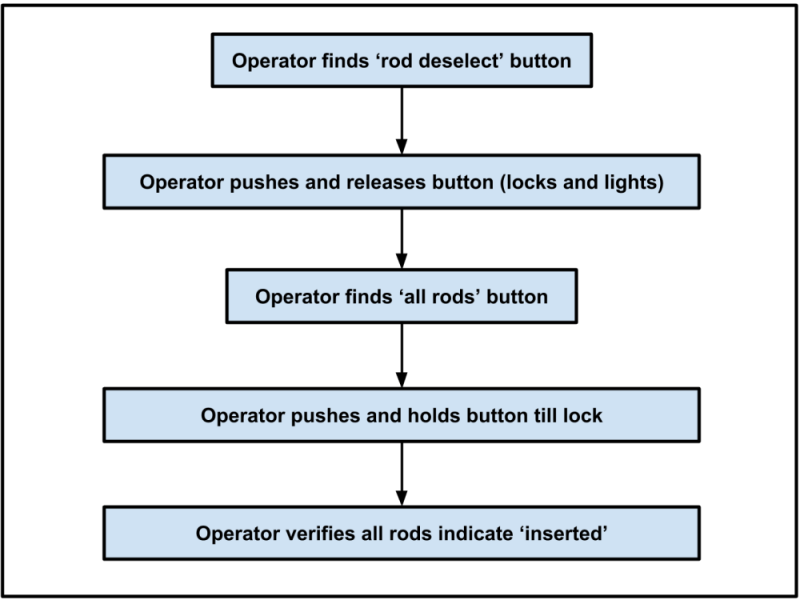
\includegraphics[width=0.80\textwidth]{hra_rods.inserted.jpg}
%        \caption{}
    \end{figure}
\end{frame}


\begin{frame}{Task analysis validates operator actions}
    \begin{enumerate}[series=outerlist,topsep=0pt,itemsep=21pt,leftmargin=*,label=(\arabic*)]
        \item[]Figure 12.1
        \item[]Operators must validate the sequence
        \item[]A lot to do in just one \acs{npp}
        \item[]Why do we need to be so detailed?
        \item[]What would cause a failure?
    \end{enumerate}
\end{frame}


\begin{frame}[plain]{}
    \centering\LARGE\textbf{Picture break}
\end{frame}


\begin{frame}{}
    \begin{figure}
        \centering
        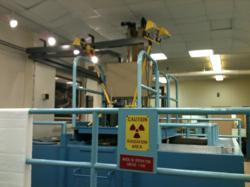
\includegraphics[width=0.80\textwidth]{wpi.reactor1.jpg}
%        \caption{}
    \end{figure}
\end{frame}


\begin{frame}{}
    \begin{figure}
        \centering
        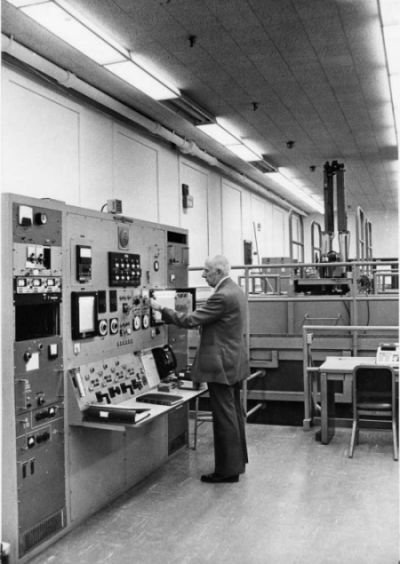
\includegraphics[width=0.40\textwidth]{wpi.reactor2.jpg}
%        \caption{}
    \end{figure}
\end{frame}


\begin{frame}{Visually depict each task as a failure with applicable recovery actions}
    \begin{enumerate}[series=outerlist,topsep=0pt,itemsep=18pt,leftmargin=*,label=(\arabic*)]
        \item[]\acs{hra} model needs to visually depict each task as a failure with applicable recovery actions
        \item[]Potential human errors and their mechanisms
        \item[]Recovery paths if error occurs
        \item[]Quantify error (frequency)
        \item[]What would be the errors and recovery acts for the \acs{scr} rods sequence? 
        \item[]Could make an event tree or fault tree from this
        \item[]Though fault tree would be just one and gate (figure 12.3) for failure to verify rod insertion
    \end{enumerate}
\end{frame}


\begin{frame}[plain]{}
    \centering\LARGE\textbf{Human error probability}
\end{frame}


\addtocounter{framenumber}{-1}
\begin{frame}{Human error probability is difficult to quantify}
    \begin{enumerate}[series=outerlist,topsep=0pt,itemsep=21pt,leftmargin=*,label=(\arabic*)]
        \item[]Because people generally behave stupidly even sober
        \item[]Or, different responses are elicited by people in the same environment
        \item[]What would be examples of human errors that could be quantified?
        \item[]Astronaut behavior in normal conditions and critical conditions
        \item[]Psychological stress
    \end{enumerate}
\end{frame}


\begin{frame}{Performance shaping factors account for human response to stressors}
    \begin{enumerate}[series=outerlist,topsep=0pt,itemsep=3pt,leftmargin=*,label=(\arabic*)]
        \item[]hot/cold  
        \item[]noise level   
        \item[]light level (my office is dark)  
        \item[]vibration  
        \item[]ergonomics
        \item[]experience and training
        \item[]management
        \item[]time
        \item[]stress
        \item[]equipment design/human machine interface
    \end{enumerate}
\end{frame}


\begin{frame}[plain]{}
    \centering\LARGE\textbf{Now, we need to figure out probabilities}
\end{frame}


\addtocounter{framenumber}{-1}
\begin{frame}{Each task then would have an associated probability}
    \begin{enumerate}[series=outerlist,topsep=0pt,itemsep=15pt,leftmargin=*,label=(\arabic*)]
        \item[]\href{https://uidaho.pressbooks.pub/riskassessment/chapter/human-reliability-analysis/}{Handbook of Human Reliability Analysis with Emphasis on Nuclear Power Plant Applications}
        \item[]`The completion cue or sign for the task or activity is simple and unambiguous.'
        \item[]Not identifying buttons may be due to labeling, or whether they're lit up
        \item[]Also need to establish what everything looks like under normal operations
        \item[]\acsp{npp} have certain instrumentation and processes not found in other facilities
        \item[]Now what happens when control panels are digitized?  
    \end{enumerate}
\end{frame}


\begin{frame}{Increasing complexity with human error happens fast}
    \begin{enumerate}[series=outerlist,topsep=0pt,itemsep=21pt,leftmargin=*,label=(\arabic*)]
        \item[]\href{https://uidaho.pressbooks.pub/riskassessment/chapter/human-reliability-analysis/}{\acs{trp} tables}
        \item[]Operator fails to find Rod Deselect button = 0.003 Table 20-12 item 2
    \end{enumerate}
\end{frame}


\begin{frame}{Obtaining human error data is really the same as equipment failure rates}
    \begin{enumerate}[series=outerlist,topsep=0pt,itemsep=21pt,leftmargin=*,label=(\arabic*)]
        \item[]Search historical data for the task
        \item[]Expert advice
        \item[]We could ask people who have worked on manipulators for hot cells
        \item[]Simulations of the activity can be performed and data collected 
        \item[]Now, there are tons of \acsp{pra} to study for related activities
        \item[]Delphi studies
    \end{enumerate}
\end{frame}


\begin{frame}{Performance shaping factors affect human error}
    \begin{enumerate}[series=outerlist,topsep=0pt,itemsep=3pt,leftmargin=*,label=(\arabic*)]
        \item[]hot/cold  
        \item[]noise level   
        \item[]light level (my office is dark)  
        \item[]vibration  
        \item[]ergonomics
        \item[]experience and training
        \item[]management
        \item[]time
        \item[]stress
        \item[]equipment design/human machine interface
    \end{enumerate}
\end{frame}


\begin{frame}{How can we reduce human error?}
    \begin{enumerate}[series=outerlist,topsep=0pt,itemsep=15pt,leftmargin=*,label=(\arabic*)]
        \item[]Is there a procedure that is followed?  
        \item[]Pre-start checklist, log, and shutdown for WPI reactor  
        \item[]If there is an error in reactor operation, the checklist could show that  
        \item[]Procedures have to be memorized though
        \item[]Is there time pressure to complete the sequence?  
        \item[]\acs{scr} actions need to be completed in about 3 minutes
        \item[]So you need to know your actions  
        \item[]Familiarity can lead to cutting corners and errors  
    \end{enumerate}
\end{frame}


\begin{frame}[plain]{}
    \centering\LARGE\textbf{Common cause}
\end{frame}


\addtocounter{framenumber}{-1}
\begin{frame}{Avoid dependencies}
    \begin{enumerate}[series=outerlist,topsep=0pt,itemsep=15pt,leftmargin=*,label=(\arabic*)]
        \item[]Dependence is relationship between tasks \href{https://uidaho.pressbooks.pub/riskassessment/chapter/human-reliability-analysis/}{Chapter 10 NUREG}
        \item[]Now we have a new problem with reactor controls going digital
        \item[]New cyberattacks from new equipment  
        \item[]\href{https://www.sciencedirect.com/science/article/abs/pii/S0149197023001774}{How do operators identify a cyberattack?}
        \item[]How do they respond?  
        \item[]We need to make sure we identify the most critical procedures to analyze
        \item[]Don't want to waste money on simple tasks
    \end{enumerate}
\end{frame}


\begin{frame}[plain]{}
    \centering\LARGE\textbf{\acs{haz}}
\end{frame}


\addtocounter{framenumber}{-1}
\begin{frame}{\acs{haz} identifies hazards without waiting for an accident to occur}
    \begin{enumerate}[series=outerlist,topsep=0pt,itemsep=21pt,leftmargin=*,label=(\arabic*)]
        \item[]Developed by Imperial Chemical Industries in early 1960s
        \item[]Not only for safety, but efficient operations
        \item[]Accidents caused by deviations from design/operating intentions
        \item[]Identifying potential hazards and operability problems caused by deviations from the design intent of both new and existing process plants
        \item[]Essential feature to review process drawings and/or procedures
    \end{enumerate}
\end{frame}


\begin{frame}{Identify all possible deviations from normal operation and associated hazards}
    \begin{enumerate}[series=outerlist,topsep=0pt,itemsep=7pt,leftmargin=*,label=(\arabic*)]
        \item[]`What if' analysis for system parameters  
        \item[]What if `temperature' of `reactor' `rises'?
        \item[]System realization of perturbation (or sensitivity analysis)
        \item[]Requires flow model of operating plant  
        \item[]So this is not something done too early on in design phases  
        \item[]But can affect design  
        \item[]Later on in the life cycle if facility upgrades/retrofits have been made  
        \item[]For use with \acs{pha} \& \acs{fma} and provides input to event trees too  
        \item[]Can offer some options to mitigate hazards
        \item[]\acs{haz} seems to me to be a limited fit for industrial facilities/reactors
    \end{enumerate}
\end{frame}


\begin{frame}{\acs{haz} is a structured and systematic technique for examining a defined system}
    \begin{enumerate}[series=outerlist,topsep=0pt,itemsep=21pt,leftmargin=*,label=(\arabic*)]
        \item[]Identify potential hazards in the system  
        \item[]Identifying potential operability problems with the system, causes of operational disturbances, and production deviations
        \item[]Ensure that all relevant deviations of process parameters are evaluated  
        \item[]Causes of deviations are human error, equipment failure, external events
        \item[]Deviation = Guideword + Parameter
    \end{enumerate}
\end{frame}


\begin{frame}{Operability is any process inside the design envelope that would cause a shutdown}
    \begin{enumerate}[series=outerlist,topsep=0pt,itemsep=21pt,leftmargin=*,label=(\arabic*)]
        \item[]Where a shutdown could possibly lead to a violation of environmental, health or safety regulations or negatively impact profitability
        \item[]Also called licensing basis envelope
        \item[]More about system operation than safety
    \end{enumerate}
\end{frame}


\begin{frame}{\acs{haz} deals with the identification of potential deviations from the design}
    \begin{enumerate}[series=outerlist,topsep=0pt,itemsep=17pt,leftmargin=*,label=(\arabic*)]
        \item[]Intent, examination of causes, and assessment of consequences
        \item[]Improve operating procedures or when modifying plant 
        \item[]Identify possible improvements where accident rate is abnormally high 
        \item[]Time consuming and can be tedious (Theo from Simplot)
        \item[]Generates many failure events with insignificant risk  
        \item[]Again, can miss common cause failures
        \item[]Tends to ignore contributions that can be made by operator interventions 
    \end{enumerate}
\end{frame}


\begin{frame}{\acs{haz} has a logical structure like event and fault trees}
    \begin{enumerate}[series=outerlist,topsep=0pt,itemsep=21pt,leftmargin=*,label=(\arabic*)]
        \item[]Flowing/process items are `entities' (study nodes)
        \item[]Entities have characteristic properties known as `attributes'
        \item[]Analysis based on possible deviations of attribute values (sensitivities)
        \item[]`Guide words' used to guide the analysis and designed to capture dimensions of variation
    \end{enumerate}
\end{frame}


\begin{frame}[plain]{}
    \centering\LARGE\textbf{Flowchart}
\end{frame}


\addtocounter{framenumber}{-1}
\begin{frame}{}
    \begin{figure}
        \centering
        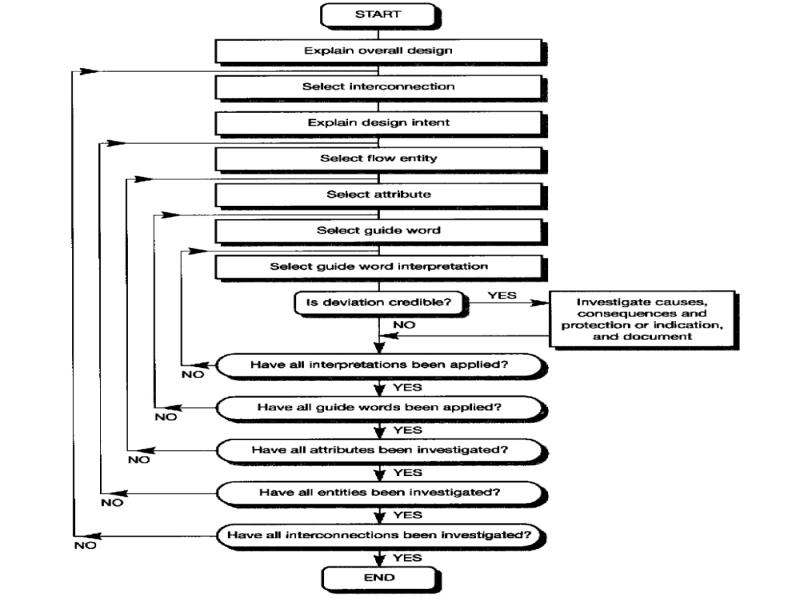
\includegraphics[width=0.80\textwidth]{hazop_flowchart.jpg}
%        \caption{}
    \end{figure}
\end{frame}


\begin{frame}{}
    \begin{figure}
        \centering
        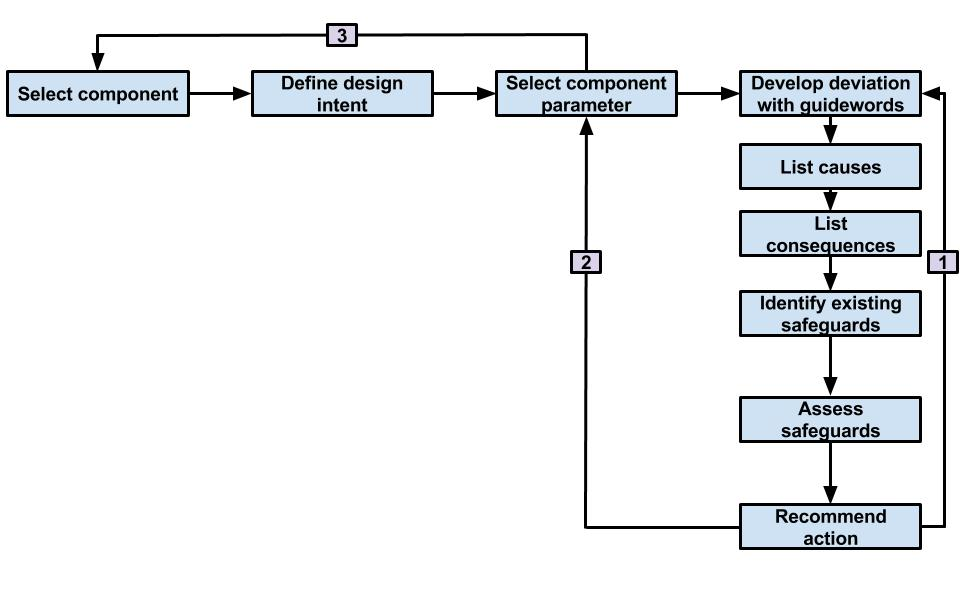
\includegraphics[width=0.80\textwidth]{hazop.loop.jpg}
%        \caption{}
    \end{figure}
\end{frame}


\begin{frame}[plain]{}
    \centering\LARGE\textbf{Flash drum example}
\end{frame}


\addtocounter{framenumber}{-1}
\begin{frame}{}
    \begin{figure}
        \centering
        \href{https://uidaho.pressbooks.pub/riskassessment/chapter/hazop/}{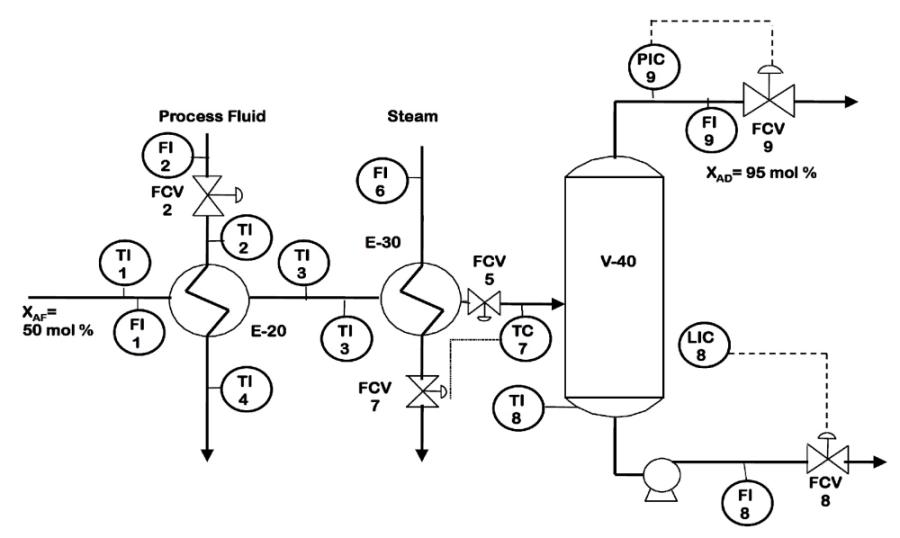
\includegraphics[width=0.90\textwidth]{hazop_flash.drum.jpg}}
%        \caption{}
    \end{figure}
\end{frame}


\begin{frame}{\acs{haz} analysis process for flash drum}
    \begin{enumerate}[series=outerlist,topsep=0pt,itemsep=1pt,leftmargin=*,label=(\arabic*)]
        \item Select component -- Flash drum
            \vspace{0.07in}
        \item Define design intent -- The flash drum separates light and heavy materials
            \vspace{0.07in}
        \item Select component parameter -- Pressure
            \vspace{0.07in}
        \item[(4a)] Develop deviation with \href{https://uidaho.pressbooks.pub/riskassessment/chapter/hazop/}{guidewords}
        \item[]More/high pressure
            \vspace{0.07in}
        \item[(4b)] List causes -- Valve is stuck closed; Feed temperature too high 
        \item[]Within or outside boundary  
        \item[]Derived from independent variables
            \vspace{0.07in}
        \item[(4c)] List consequences -- Explosion  
        \item[] Process hazards  
        \item[] Operability problems 
    \end{enumerate}
\end{frame}


\begin{frame}{\acs{haz} analysis process for flash drum}
    \begin{enumerate}[series=outerlist,topsep=0pt,itemsep=1pt,leftmargin=*,label=(\arabic*)]
        \item[(4d)]Identify existing safeguards -- Temperature control; Pressure control 
        \item[]Safeguards reduce risk
            \vspace{0.15in}
        \item[(4e)]Assess safeguards -- Are the controls adequate? No.
            \vspace{0.15in}
        \item[(4f)]Recommend action -- Relief valve; Alarm
        \item[]Action to remove cause, mitigate consequence
            \vspace{0.15in}
        \item[]Return to 4a until all deviations have been analyzed under the component parameter
            \vspace{0.15in}
        \item[]Return to 3 and identify new component parameter
            \vspace{0.15in}
        \item[]Return to 1 and select new component
    \end{enumerate}
\end{frame}


\begin{frame}[plain]{}
    \centering\LARGE\textbf{Safeguards}
\end{frame}


\addtocounter{framenumber}{-1}
\begin{frame}{There are five types of safeguards}
    \begin{enumerate}[series=outerlist,topsep=0pt,itemsep=1pt,leftmargin=*,label=(\arabic*)]
        \item[]\textbf{IDENTIFY}
        \item[]alarm instrumentation  
        \item[]human operator detection  
            \vspace{0.07in}
        \item[]\textbf{COMPENSATE}
        \item[]automatic control system
            \vspace{0.07in}
        \item[]\textbf{PREVENT}
        \item[]inert blanket gas in storage of flammable substances -- AP1000 water blanket
            \vspace{0.07in}
        \item[]\textbf{DESCALATION}
        \item[]trip of the activity -- \acs{scr}
            \vspace{0.07in}
        \item[]\textbf{RELIEVE}
        \item[]pressure safety valves
        \item[]vent systems
    \end{enumerate}
\end{frame}


\begin{frame}[plain]{}
    \centering\LARGE\textbf{Record keeping}
\end{frame}


\addtocounter{framenumber}{-1}
\begin{frame}{You can set up a chart}
    \begin{enumerate}[series=outerlist,topsep=0pt,itemsep=21pt,leftmargin=*,label=(\arabic*)]
        \item[]\href{https://red-bag.com/imageslib/BN-EG-UE105_02.pdf}{Recording sheet}
        \item[]\href{http://www.ehsdb.com/resources/Imges-3/Images-3/hazop-15.JPG?timestamp=1436341480548}{Chemical reactor}
        \item[]\href{http://www.ehsdb.com/resources/Imges-3/Images-3/hazop-18.JPG?timestamp=1436342662934}{Heat exchanger}
        \item[]\href{http://group10integratedprojectmay15.weebly.com/hazop-and-pid.html}{\acs{pid} schematic}
    \end{enumerate}
\end{frame}


\begin{frame}[plain]{}
    \centering\LARGE\textbf{Pyroprocessing}
\end{frame}


\addtocounter{framenumber}{-1}
\begin{frame}{}
    \begin{figure}
        \centering
        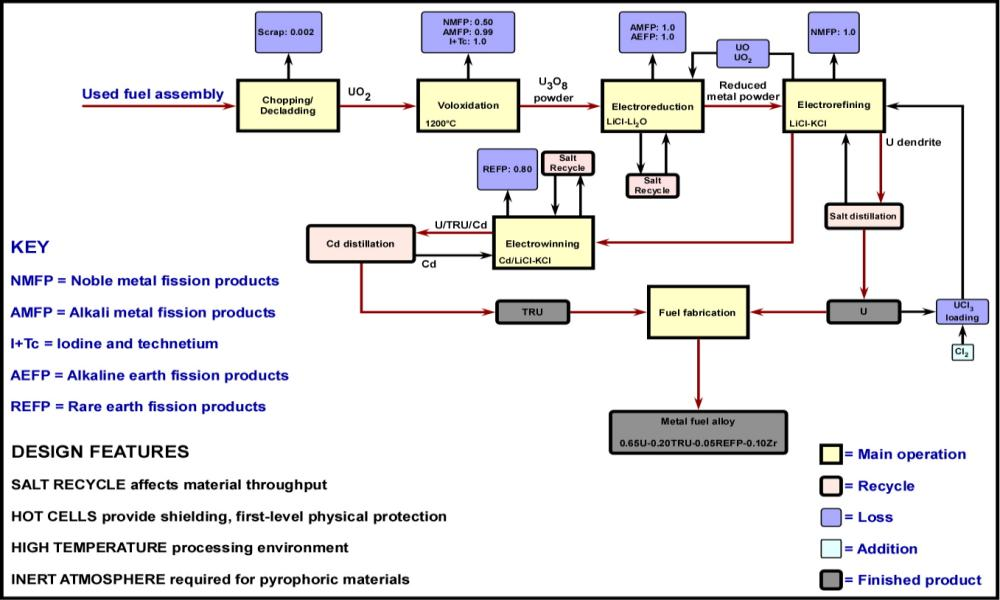
\includegraphics[width=0.80\textwidth]{pyroprocessing.flowsheet.jpg}
%        \caption{}
    \end{figure}
\end{frame}


\begin{frame}{\acs{haz} analysis process for pyroprocessing injection casting}
    \begin{enumerate}[series=outerlist,topsep=0pt,itemsep=1pt,leftmargin=*,label=(\arabic*)]
        \item Select component -- Injection casting
            \vspace{0.05in}
        \item Define design intent -- Manufacture metal fuel slugs that contain U+TRU
            \vspace{0.05in}
        \item Select component parameter -- Temperature
            \vspace{0.05in}
        \item[(4a)] Develop deviation with \href{https://uidaho.pressbooks.pub/riskassessment/chapter/hazop/}{guidewords}
        \item[]Less temperature
            \vspace{0.05in}
        \item[(4b)] List causes -- Heater malfunction; Fails to start; Starts late; Power source failure
        \item[]Within or outside boundary  
        \item[]Derived from independent variables
            \vspace{0.05in}
        \item[(4c)] List consequences -- Metal is not totally melted; Quartz molds break; Spill liquid metal 
        \item[] Process hazards  
        \item[] Operability problems 
    \end{enumerate}
\end{frame}


\begin{frame}{\acs{haz} analysis process for pyroprocessing injection casting}
    \begin{enumerate}[series=outerlist,topsep=0pt,itemsep=1pt,leftmargin=*,label=(\arabic*)]
        \item[(4d)]Identify existing safeguards -- Unknown
        \item[]Safeguards reduce risk
            \vspace{0.15in}
        \item[(4e)]Assess safeguards -- None
            \vspace{0.15in}
        \item[(4f)]Recommend action -- Instrumentation; Human detection
        \item[]Action to remove cause, mitigate consequence
            \vspace{0.15in}
        \item[]Return to 4a until all deviations have been analyzed under the component parameter
            \vspace{0.15in}
        \item[]Return to 3 and identify new component parameter
            \vspace{0.15in}
        \item[]Return to 1 and select new component
    \end{enumerate}
\end{frame}


\begin{frame}{Select temperature}
    \begin{enumerate}[series=outerlist,topsep=0pt,itemsep=21pt,leftmargin=*,label=(\arabic*)]
        \item[]\textbf{Deviation} -- LESS+TEMPERATURE --- Low temperature
        \item[]\textbf{Causes} -- Heater fails to start; Heater starts late; Power source not available
        \item[]\textbf{Consequences} -- Metal not melted; Quartz molds break; Molten TRU spill
        \item[]\textbf{Protection} -- Unknown
        \item[]\textbf{Action} -- Install temperature indicator; Human detection; Positive injection operation
    \end{enumerate}
\end{frame}


\begin{frame}{Select time}
    \begin{enumerate}[series=outerlist,topsep=0pt,itemsep=21pt,leftmargin=*,label=(\arabic*)]
        \item[]\textbf{Deviation} -- LESS+TIME --- Short injection time
        \item[]\textbf{Causes} -- Operator error; Motor trip
        \item[]\textbf{Consequences} -- Not enough metal injected into molds; Waste of material
        \item[]\textbf{Protection} -- Unknown
        \item[]\textbf{Action} -- Install timer; Human detection; Positive mold removal operation
    \end{enumerate}
\end{frame}


\begin{frame}[plain]{}
    \centering\LARGE\textbf{Advantages}
\end{frame}


\addtocounter{framenumber}{-1}
\begin{frame}{What's good about \acs{haz}}
    \begin{enumerate}[series=outerlist,topsep=0pt,itemsep=15pt,leftmargin=*,label=(\arabic*)]
        \item[]Considers more than failure accidents  
        \item[]Process and operation deviations
        \item[]Can identify new hazards  
        \item[]Not limited to previously identified hazards
        \item[]A simple method that can uncover complex accidents  
        \item[]Applicable to new designs and new design features
    \end{enumerate}
\end{frame}


\begin{frame}[plain]{}
    \centering\LARGE\textbf{Disadvantages}
\end{frame}


\addtocounter{framenumber}{-1}
\begin{frame}{What are the drawbacks?}
    \begin{enumerate}[series=outerlist,topsep=0pt,itemsep=11pt,leftmargin=*,label=(\arabic*)]
        \item[]Requires detailed plant information  
        \item[]Flowsheets, piping and instrumentation diagrams, plant layout
        \item[]Tends to result in protective devices rather than real design changes
        \item[]Relies very heavily on judgment of engineers (and?)
        \item[]Unusual to consider deviations for systemic factors  
        \item[]Organizational, managerial factors, management systems
        \item[]Difficult to apply to software (not really an automated procedure)
        \item[]Human behavior reduces to compliance/deviation from procedures  
        \item[]Does not account for human performance factors
    \end{enumerate}
\end{frame}


\begin{frame}[plain]{}
    \begin{figure}
        \centering
        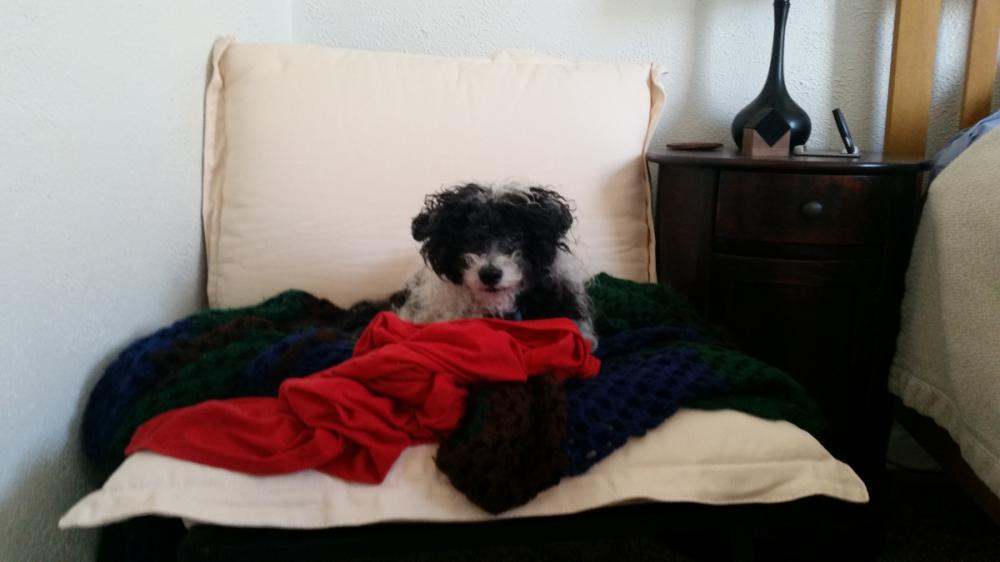
\includegraphics[width=0.85\textwidth]{final.jpg}
%        \caption{}
    \end{figure}
\end{frame}


%%%%%%%
%\begin{frame}{}
%    \begin{columns}
%
%        \begin{column}{0.50\textwidth}
%            \begin{enumerate}[series=outerlist,topsep=0pt,itemsep=21pt,leftmargin=*,label=(\arabic*)]
%                \item[]
%                \item[]
%            \end{enumerate}
%        \end{column}
%
%        \begin{column}{0.50\textwidth}
%            \begin{enumerate}[series=outerlist,topsep=0pt,itemsep=21pt,leftmargin=*,label=(\arabic*)]
%                \item[]
%                \item[]
%            \end{enumerate}
%        \end{column}
%
%    \end{columns}
%\end{frame}

%    \begin{figure}
%        \centering
%        \includegraphics[width=0.75\textwidth]{wsc.png}
%        \caption{\acs{wsc}}
%    \end{figure}


%\begin{frame}{References}
%    \bibliographystyle{nsf}
%    \footnotesize
%    \bibliography{references}
%\end{frame}
%%%%%%%


\end{document}
